\documentclass{ujarticle}
\usepackage{moreverb}
\usepackage[dvipdfmx]{graphicx}
\title{熱伝導方程式の差分法による解法}
\begin{document}
\maketitle
\section{目的}
湯気のシミュレーションにおいて熱伝導方程式を解く必要がある。
熱伝導方程式の差分法による解法をまとめる。
\section{熱伝導方程式}
一次元の熱伝導方程式は次式で表される。
\begin{equation}
\frac{\partial T}{\partial t} = \alpha \frac{\partial^2T}{\partial^2x}
\end{equation}
$T$は温度、$\alpha$は温度伝導率であり、次式より求まる。
\begin{equation}
\alpha=\frac{\lambda}{\rho c_{p}}
\end{equation}
$\lambda$は熱伝導率、$\rho$は密度、$c_{p}$は定圧比熱である。
\section{偏導関数の近似}
差分法では偏導関数を前進差分、後退差分で次のように近似する。
\begin{equation}
\frac{\partial f}{\partial x}=\frac{f_{i+1}-f_{i}}{\Delta x}
\end{equation}
\begin{equation}
\frac{\partial f}{\partial x}=\frac{f_{i}-f_{i-1}}{\Delta x}
\end{equation}
2階の偏導関数は1階の偏導関数であるから前進差分と後退差分を用いれば次式を得られる。
\begin{equation}
\frac{\partial^2 f}{\partial^2 x} = \frac{f_{i+1}-2f_{i}+f_{i-1}}{\Delta x^2}
\end{equation}
\section{陽解法}
前進差分を用いて数値解を求める方法は陽解法と呼ばれる。
$T_{x,t}$として陽解法による差分近似式は次式になる。
\begin{equation}
\frac{T_{i,j+1} - T_{i,j}}{\Delta t} = \alpha\frac{T_{i+1,j}-2T_{i,j}+T_{i-1,j}}{\Delta x^2}
	\end{equation}
$T_{i,j+1}$について解くと次式になる。ここで$\gamma$は$\frac{\Delta t}{\Delta x^2}$となる。
\begin{equation}
T_{i,j+1}=\alpha \gamma T_{i+1,j} + (1-2 \alpha \gamma)T_{i,j}+\alpha \gamma T_{i-1,j}
\end{equation}

\section{陰解法}
後退差分を用いて数値解を求める方法は陰解法と呼ばれる。
差分近似式は次式となる。
\begin{equation}
\frac{T_{i,j+1}-T_{i,j}}{\Delta t} = \alpha \frac{T_{i+1,j+1}-2T_{i,j+1}+T_{i-1,j+1}}{\Delta x^2}
\end{equation}
これを整理すると次式になる。
\begin{equation}
-\alpha \gamma T_{i+1,j+1}+(1+2 \alpha \gamma)T_{i,j+1} - \alpha \gamma T_{i-1,j+1} = T_{i,j}
\end{equation}
陽解法とは異なり$T_{i,j}$から、次の時刻での$T_{i-1,j+1},T_{i,j+1},T_{i+1,j+1}$の3点を求める。
前式を行列で表すと次の式のようになる。

\[
  \left(
    \begin{array}{ccccc}
      1+2 \alpha \gamma & -\alpha \gamma  & 0 & \ldots & 0 \\
      -\alpha \gamma  & 1+2 \alpha \gamma & -\alpha \gamma & \ldots & 0 \\
       & \vdots &  & \ddots & \vdots \\
      0 & \ldots & -\alpha \gamma  & 1+2 \alpha \gamma & -\alpha \gamma \\
      0 & \ldots & 0 &  -\alpha \gamma  & 1+2 \alpha \gamma
    \end{array}
  \right)
  \left(
  	\begin{array}{c}
  		T_{1,j+1} \\ T_{2,j+1} \\ \ldots \\ T_{M-1,j+1} \\ T_{M,j+1} 
  	\end{array}
  \right)
  =
  \left(
  	\begin{array}{c}
 		T_{1,j} \\ T_{2,j} \\ \ldots \\ T_{M-1,j} \\ T_{M,j} 
  	\end{array}
  \right)
\]

前式の連立一次方程式を数値解法によって解く。このとき行列の$T_{i,j+1}$と$T_{M,j+1}$には境界条件を設定する。

陰解法を用いてガウスサイデル法により一次元の熱伝導方程式を解いたPythonのプログラム例とその結果を以下に示す。
\verbatimtabinput{heat_3.py}
\begin{figure}[h]
	\begin{center}
		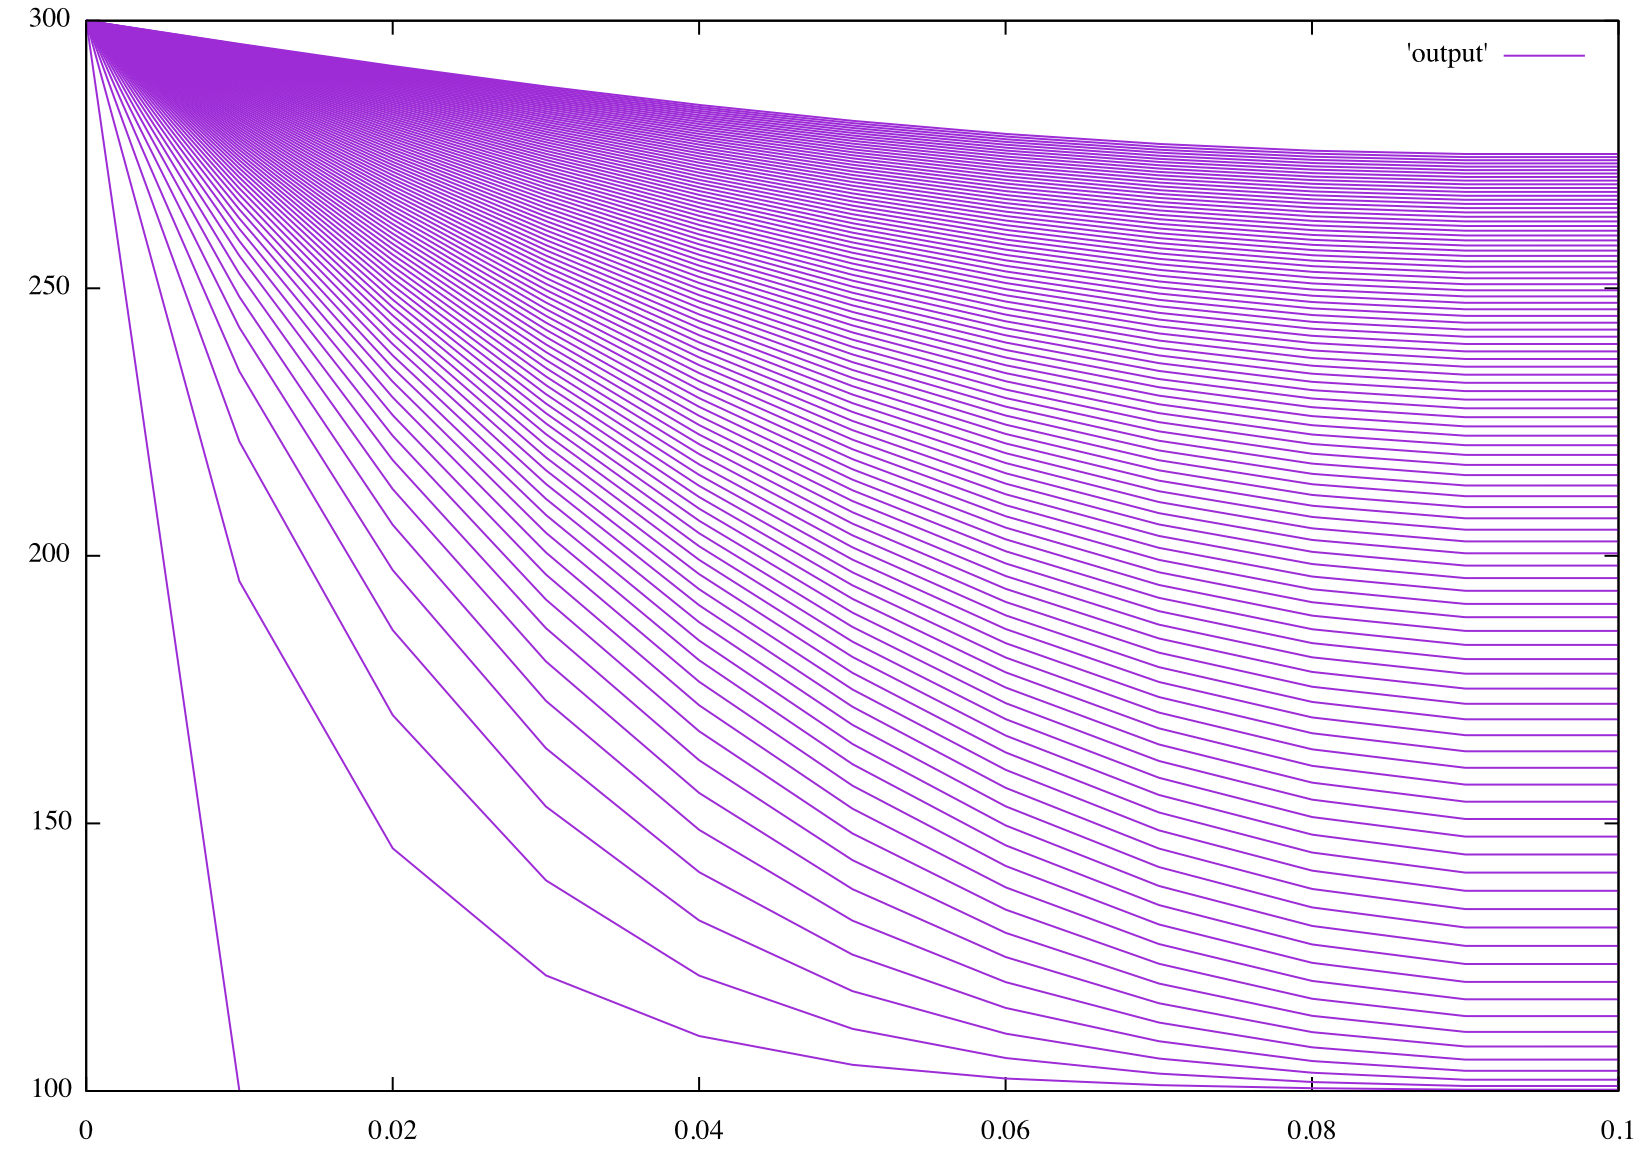
\includegraphics[width=100mm]{heat.png}
	\end{center}
\end{figure}

\end{document}